\documentclass[11pt]{article}
\usepackage{float}
\usepackage{fullpage}
\usepackage{amssymb}
\usepackage{amsthm}
\usepackage{color}
\usepackage{enumerate}
\usepackage{amsmath}
\usepackage{dirtytalk}
\usepackage{graphicx}
\usepackage[margin=0.8in]{geometry}
\usepackage{listings}
\usepackage{framed}
\lstset{
	language=C,
	basicstyle=\scriptsize\ttfamily,
	commentstyle=\ttfamily\color{green},
	numbers=left,
	numberstyle=\ttfamily\color{blue}\footnotesize,
	stepnumber=1,
	numbersep=5pt,
	backgroundcolor=\color{white},
	showspaces=false,
	showstringspaces=false,
	showtabs=false,
	frame=single,
	tabsize=2,
	captionpos=b,
	breaklines=true,
	breakatwhitespace=false,
	title=\lstname,
	escapeinside={},
	keywordstyle={},
	morekeywords={}
}

\setcounter{secnumdepth}{0}

\begin{document}

\title{Report: ARM11 Project \\ Group 8}
\author{Elliot Grenwood, Elyas Addo, Florian Emile, Nana Asiedu-Ampem}

\maketitle

\section{Introduction}
This report covers the completion of Group 8's ARM11 Project, specifically Parts II - IV: Assembler; General Purpose Input/Output on a Raspberry Pi; our chosen extension. The assembler program, like the emulator, is written in C. Part of the extension is also written in C, and the other part in the ARM11 assembly language. In this report we will also discuss the organisation and communication of the group.

\section{Part II - Assembler}
The assembler can be split into 6 subtasks:\newline

\begin{lstlisting}
// SETUP
setUpIO(inputFile, outputFile, pProgram);

// RUN PROGRAM
/* create an array of tokens
 * Token is composed of two fields - the original string and the token type
 */
tokenise(inputFile);
// map labels to addresses
resolveLabelAddresses(pProgram);
// call the respective parse function depending on opcode (string field in token)
parseProgram(tokenArray);
/* generate binary instruction in big endian by computing relevant flags and
/* binary representation for each argument of opcode
 */
generateInstrunction(opcode);
//ouput instruction in little endian to ouputFile
outputData();

// DEALLOCATION
closeFiles();
freeInternalMemorySpaces();

}
\end{lstlisting}

Using assembly files in a provided testsuite, the \texttt{./assemble} outputs were compared to the expected outputs to ensure the program function correctly. We also built files for testing data structures, such as the queue - this ensured we knew this unit of the program was working as we wanted to, affording us the opportunity to use its functions freely in our program.

\section{Part III - GPIO (General Purpose Input/ Output)}
Since inputs and outputs required no special instructions, \texttt{./assemble} needed do amending, all updates were made in \texttt{./emulate}. Constants were added which contain the GPIO set/clear area addresses used to alter the output of pins. Three more constants were created to contain the GPIO status addresses that modify the state of each pin (input or output). Extra memory structures were created for these addresses to refer to, this is how the states are manipulated.\newline

\noindent Deciding how to implement this extra part of the memory was a challenge. Originally the existing RAM structure was extended, however, this was prone to errors with arithmetic operations. This is why it was decided to create a separate structure for the GPIO pins.\newline

\noindent In order to test our understanding of how the Raspberry Pi handled outputs, a simple program to flash an LED was created. This test was successful, below is the code used. Note that the comments were added after the program was assembled.

\lstinputlisting{gpio.s}

\section{Part IV - Extension}

Our chosen extension has 4 parts: changing the functionality of \texttt{mov r15, r14} to allow returns from function calls; allowing the use of comments in an assembler file being passed into our assembly program; creating a 3 bit binary counter in assembly language; creating a IR-based counter. \newline

%all have description, design, problems, testing, USAGE
\subsection{Implementing \texttt{mov r15, rn}}
In order to use functions, a program can create its own stack structure in memory. This allows the program to store the derived return address and then branch to a function. However, in order to return from a function the PC must store the return address whilst maintaining the pipeline effect. The ARM11 architecture already has a \texttt{mov PC, rn} command which braches automatically so \texttt{./assemble} needed no changing. However, to test the function we have improved the \texttt{mov} instruction in the emulator to allow the PC to store in a chosen address and then branch immediately. again this was very little challenge as it simply involved a small if statement checking the destination resister.

\subsection{Comments}
The ability to write comments alongside instructions is a useful feature. It can improve the clarity of assembly code which allows for easier maintainance. Comments begin with a semi-colon and finish at the end of the line. They can be placed either on an empty line or at the end of an instruction. For a new-line and end-of-line comments there are 3 types to test for: a blank comment with no text (e.g. \texttt{;}), a comment with no spaces at the start (e.g. \texttt{;comment}), a comment with spaces after the start (e.g. \texttt{; comment}).\newline

\noindent Since comments only exist in an assembly file, only the assembler program had to be edited. The \verb|tokenise()| function was amended to check for a \texttt{;} at the beginning of a token, and if one is found, start reading the next line. Although the comment update was implemented by a member of the group who didn't work on the tokeniser, change was easily made due to the clarity of the original design.\newline

\noindent Figure 1 below shows the \texttt{./emulate} output for the \texttt{commentTest} program assembled with and without the comments. We also used our assembler on the original test suite to ensure the feature didn't affect any other element of the program.
\lstinputlisting{commentTest.s}

\begin{figure}[H]
	\centering
	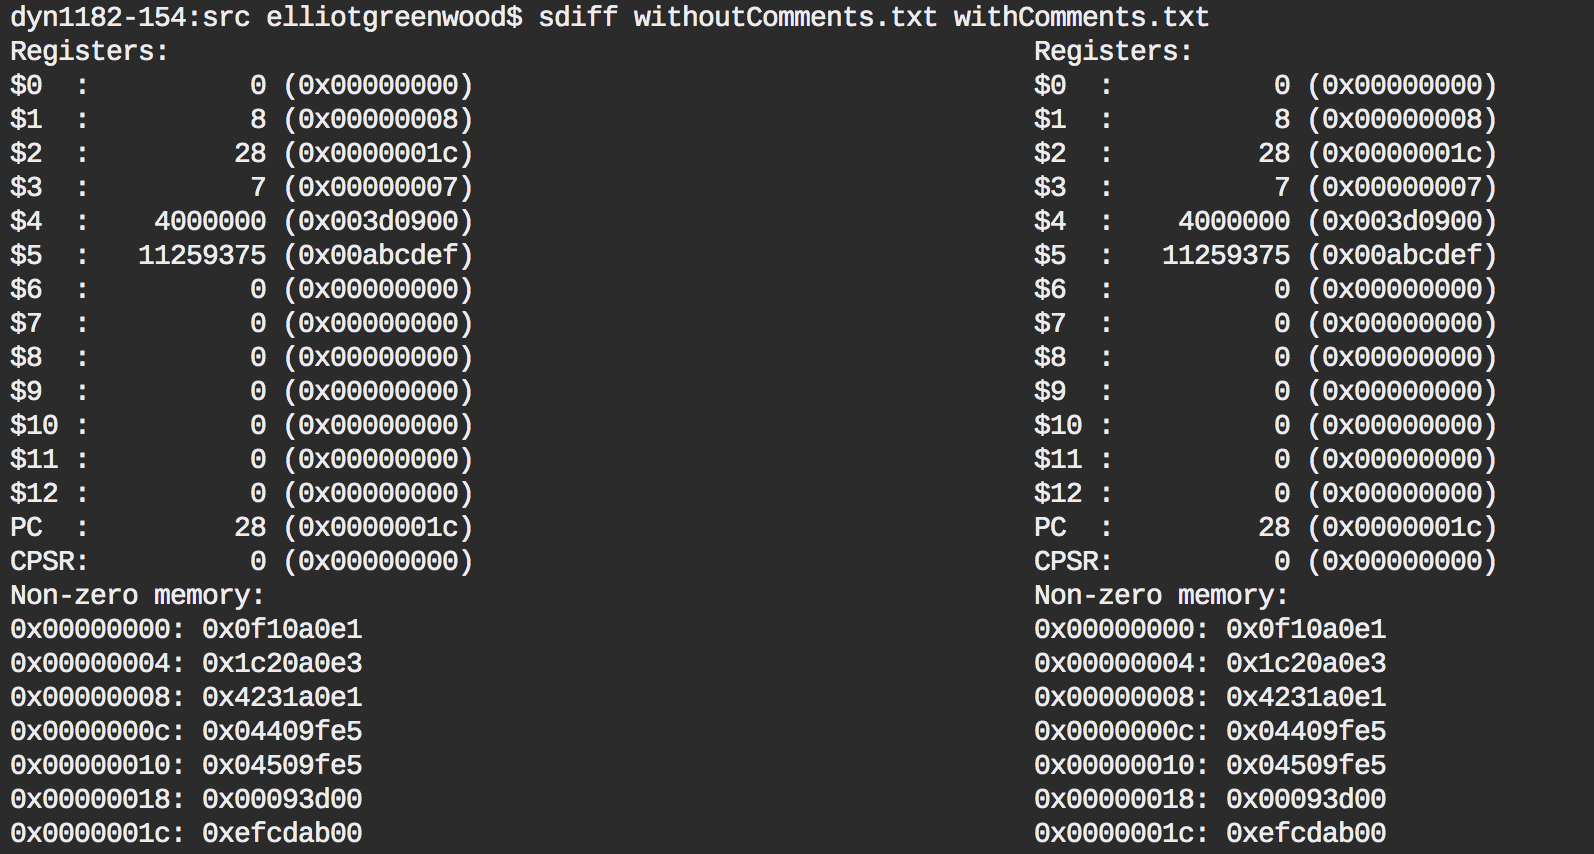
\includegraphics[scale = 0.5]{commentTest}
	\caption{No difference between outputs without comments (left) and with comments}
\end{figure}

\subsection{3 Bit Binary Counter}
 Three LEDs are connected to the Raspberry Pi which represent the bit pattern (i.e. The LED being on represents a 1). The assembly program written counts from 0 to 7 at regular intervals. The required pins are then cleared and set by the program to control the LEDs. An issue encountered was the choice of pins to use to increase the simplicity of the program, since when the Raspberry Pi is first turned on, some pins are used for certain functions. Since these were just initialisation usages, it was decided that there was no issue operating these pins.

 The program was first run by our emulator to make sure that the program did set pins as expected, it was then run on the Raspberry Pi. Both tests were passed.

\subsection{IR-Based Counter}
This part of the extension is essential a way of registering motion or obstructions and carrying out an event related to whatever situation this system is used in. The set up (of a photo gate) involves an infrared LED powered and lined up with a phototransistor which is set as an input device to the Raspberry Pi. The relevant function is called as soon as the IR beam is interrupted, the incrementing of a counter has been chosen the function for demonstration.\newline

\noindent This photo gate can be used for a variety of applications such as an alarm system, speed detection (when used with a timer) and simple games that require objects to reach a certain point.\newline



\section{Reflection of working in a group}
\subsection{Elliot Greenwood}

I found working in a programming group to be quite different to what I had imagined. Mostly the fact I find it difficult not to get carried away writing all the code, and knowing where certain functions were implemented, or if they had been implemented yet. Though this could have been solved by creating header files to begin with, and using that as a map of our program. \newline

Overall my strengths are in planning and organisation and the C language. Due to the fact I enjoy organsing I felt I would be good as team leader, it also meant our team was always on top of their work, they knew where in the project they should be, and what their path for the rest of the project should be; this was noted by a couple of my team members in the WebPA. I feel I picked up the C language relatively quickly and to a high enough standard for me to not be worrying about syntax whilst writing the program. Although, whilst I had encapsulated a lot of the program I think some parts may have been poorly organised. I'm also sure that with some smarter thinking a \say{neater} solution could have been implemented in the section I worked on, Part II: Assembler. \newline

I feel my main two weaknesses were my obsessional nature and stubbornness. A lot of the time I would take over a piece of work that could have been divided up, simply because I wanted to do it; whether it be because it seemed fun, a challenge or I had thought up a different way of approaching it. This was both frustrating for the team and meant I was working for an unnecessary amount of time. I was not as willing to accept the thought processes of the other team members, this led to errors taking longer to solve than they should. It also showed me that I can be quite haphazard when debugging my errors.

\subsection{Elyas Addo}
\subsection{Florian Emile}
I thought that the most challenging part of the project would have been writing
in assembly. However coding the assembler in C was the trickiest as C was new to
me and the tasks in assembly were straightforward. I had to get used to drawing
flowcharts and writing pseudo codes for part II as it made my task easier.

I found my programming skills were not on par with those of my team members. I
verified if I understood the concepts before coding. I kept my team leader
informed of my progress as I made it easier for him to help me. When I was
working on a task with someone, I was always open to his suggestions since we
can find what we think is the best solution faster.

In a different team, I would keep my team (especially team leader) informed of
my progress in the task at hand I would also like to be more independent when I
am assigned an individual task.

\subsection{Nana Asiedu-Ampem}
This is one of the first programing group projects I have participated in and I feel it has been a very enlightening experience. I used to struggle greatly with working with Git and resolving merge conflicts, but after this project I feel more comfortable with sharing code using Git repositories. I thought that I may struggle merging my code with my teammate's code, but I managed to create effective modular functions that were easy to use. My major problem was that I didn't have sufficient knowledge of C before I started to code the emulator. This led me to make poor implementations of a few functions because of my lack of understanding of C's many libraries. This also wasted a lot of time as I had to learn C as I was programming. In future I will ensure to prepare my skills for any projects or tasks I am required to complete. \newline

\subsection{Group Reflection}

\end{document}
